
\subsection*{Partie A}

\paragraph{1.}
\begin{center}
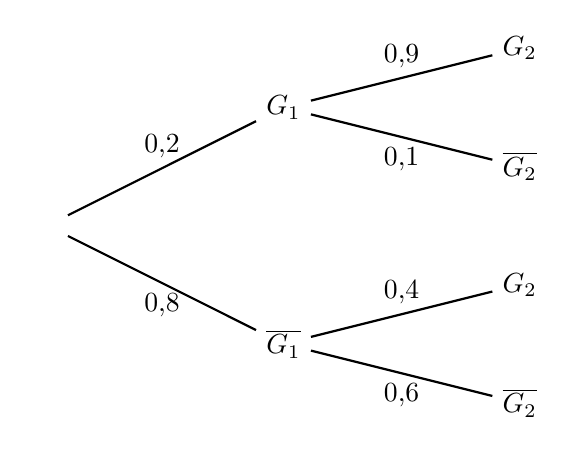
\begin{tikzpicture}[thick, scale=1.5]
\node (P_-1_0) at (-2,-1.5) {$\phantom{A}$};
\node (P_0_0) at (0,-0.5) {$G_1$};
\draw (P_-1_0) -- (P_0_0) node[midway, above] {$0{,}2$};
\node (P_1_0) at (2,-0) {$G_2$};
\draw (P_0_0) -- (P_1_0) node[midway, above] {$0{,}9$};
\node (P_1_1) at (2,-1) {$\overline{G_2}$};
\draw (P_0_0) -- (P_1_1) node[midway, below] {$0{,}1$};
\node (P_0_2) at (0,-2.5) {$\overline{G_1}$};
\draw (P_-1_0) -- (P_0_2) node[midway, below] {$0{,}8$};
\node (P_1_2) at (2,-2) {$G_2$};
\draw (P_0_2) -- (P_1_2) node[midway, above] {$0{,}4$};
\node (P_1_3) at (2,-3) {$\overline{G_2}$};
\draw (P_0_2) -- (P_1_3) node[midway, below] {$0{,}6$};
\end{tikzpicture}
\end{center}

\paragraph{2.} On a :
\[
p(G1 \cap G2) = p(G1) \times p_{G1}(G2) = 0{,}2 \times 0{,}9 = 0{,}18.
\]

\paragraph{3.} On a de même :
\[
p(\overline{G1} \cap G2) = p(\overline{G1}) \times p_{\overline{G1}}(G2) = 0{,}8 \times 0{,}4 = 0{,}32.
\]
Donc d'après la loi des probabilités totales :
\[
p(G2) = p(G1 \cap G2) + p(\overline{G1} \cap G2) = 0{,}18 + 0{,}32 = 0{,}5.
\]

\subsection*{Partie B}

\paragraph{1.}
\[
\begin{array}{|c|c|c|c|c|}
\hline
\text{Valeurs de }X & -2 & 0{,}5 & 3 & \text{Total} \\
\hline
\text{Probabilité} & 0{,}48 & 0{,}34 & 0{,}18 & 1 \\
\hline
\end{array}
\]

\paragraph{2.}
L'espérance mathématique de la variable aléatoire \(X\) est égale à :
\[
E(X) = -2 \times 0{,}48 + 0{,}5 \times 0{,}34 + 3 \times 0{,}18 = -0{,}96 + 0{,}17 + 0{,}54 = -0{,}25.
\]
Ceci signifie que sur un grand nombre de parties, un joueur perdra en moyenne 25 centimes par partie. Le jeu n'est donc pas équitable.

